\documentclass[article, 11pt]{IEEEtran}   %Document is an article, 11 pt font, and follows IEEE format

%Aqui van todos los paquetes que van a utilizar para el documento
\usepackage{hyperref}         %Uso paquete hyperref  (hiperlinks)
\usepackage{graphicx}         %Uso paquete  graphicx  (imágenes)
\usepackage{float}            %Uso paquete  float  (posicionar imágenes)
\usepackage{gensymb}          %Uso paquete  gensymb  (simbolos)
\usepackage{amsmath}          %Uso paquete  amsmath  (formulas matemáticas)
\usepackage{tikz}             %Uso paquete  tikz  (crear gráficas)
\usepackage{pgfplots}         %Uso paquete  pgfplots  (crear gráficas)
\usepackage{pgfplotstable}    %Uso paquete  pgfplotstable (regresión lineal)
\usepackage[spanish]{babel}	  %Uso paquete  babel spanish (caracteres en español)
\usepackage{lipsum}  		  %Uso paquete  lipsum (crea dummy text)

\begin{document}

%TITULO DEL REPORTE
%Las palabras inician con mayúscula excepto las preposiciones
\title{Final Project\\ Modelation and Simulation of Systems - Rocket}


%INFORMACIÓN DEL AUTOR O AUTORES
\author{\IEEEauthorblockN{José Barreno\\Luis Guzmán\\Byron García\\José Rivera}
\IEEEauthorblockA{\\Universidad Galileo, Systems Theory II\\Guatemala, Guatemala}}


% make the title area
\maketitle



%Resumen
%Esta sección es un breve resumen de los aspectos más importantes del proyecto. Se incluye el objetivo del proyecto, los hallazgos más importantes y la conclusión principal.

\begin{abstract}
\lipsum[1-1]
\end{abstract}


%INTRODUCCIÓN
%Esta sección incluye el objetivo del proyecto. Se deben incluir los %siguientes temas:
% Contexto de aprendizaje -> de que trata el proyecto, incluir el background teorico, incluir las referencias!
%El proposito del proyecto -> se incluye la hipótesis que desea probar, o la serie de preguntas que se desean contestar
%Breve resumen de la metodología utilizada y de los resultados que esperan obtener

%Link de ayuda: https://libguides.usc.edu/writingguide/introduction
\section{Introducci\'on}
\begin{otherlanguage}{english}
\section{Introduction}
When a rocket is launching, you have to control its forward acceleration and the direction it's pointing at the same time. The tricky part is that these two are highly coupled. If the thrust is slightly misaligned, it creates a pitching moment; if the pitch changes, it messes with the axial acceleration. Because of this, we can't just treat thrust and attitude as separate SISO (single-input, single-output) systems—if we do, we'll miss the crosstalk that can tank our tracking performance or make the rocket unstable. To study this, the project uses a simplified MIMO (multiple-input, multiple-output) model of a rocket moving just in the pitch plane.

To keep the math manageable, we linearized the model around a specific point during ascent. For this specific window, we're assuming small angles, constant mass and inertia, and steady aerodynamic conditions. The system has four main states: axial acceleration, pitch angle, pitch angular velocity, and nozzle deflection. We feed it acceleration and pitch commands, and measure the actual acceleration and pitch angle as outputs. The model also factors in the engine and nozzle-servo dynamics, aero damping, that destabilizing aerodynamic stiffness, and IMU feedback. The $K_1$ and $K_2$ gains are already baked into the governing equations to set the strength of the thrust and direction feedback loops.

The main goal here is to connect the math of the system back to what the rocket is actually doing physically. We're hitting it with a mix of state-space and transfer matrices, plus running stability checks, time-domain sims, frequency response, and the usual controllability and observability tests. We're mainly looking at how tweaking the control gains changes response speed, oscillations, and the interaction between the two outputs. In the frequency domain, we're checking the four input-output paths to find their bandwidths and resonance, and to see if we can actually get away with treating them as independent channels. All of this basically sets us up to pick the right gains and figure out the real-world implications of running this controller with a finite sampling time.

\end{otherlanguage}


%METODOLOGÍA
%Incluye todos los pasos que se deben seguir para llevar a cabo el experimento. Además debe incluir la justificación de la aplicación de los procedimientos. Se debe incluir cómo se obtuvo la data, qué tipo de data es y cómo fue analizada.
\section{Metodolog\'ia}
\lipsum[1-2]

%RESULTADOS
%Incluye únicamente todos los resultados obtenidos del experimentos. Pueden ser presentados en forma de tabla o gráficas. Incluye pequeños parrafos en donde es explique qué es lo que se esta presentando, o a que resultado poner atención. Sin embargo, no incluyen la interpretación de estos.
\section {Resultados}
After an analisys of the system, we found that the system models the atmosferic ascen of a rocket in the logitudinal axis, so the system start in the bloque one that has the entries of u1 and u2, for the axial aceleration and the pitch angle, those entries are passed to the central computer after pass of a converted from analog to digital to can analyse where the rocket is possioned to start making the adjustments

\subsection{Seccion A.1}
El modelo describe el movimiento de un cohete a través de un eje longitudinal que es controlado por una aceleración axial y un angulo de cabeceo para ajustar su dirección, el sistema procesa la información a través de la computadora de abordo después de haber pasado por una conversión de valores análogos a digitales para poder hacer los cálculos computacionales, reflejado en los bloques 1,2 y 3 de la figura 1, en donde se hacen los ajustes necesarios para asegurar la integridad del cohete y la trayectoria deseada, luego en los bloques 4 y 5 se envían los ajustes a través del amplificador para corregir la deflexión de la tobera lo que generara algo de inestabilidad que es registrada en el bloque 6 según que considera la dinámica del cohete, una vez obtenido estos datos, el acelerómetro y la IMU realizan sus lecturas para enviar la retroalimentación al bloque 3 que volverá a ajustar los valores hasta lograr una estabilidad esto debido a que el sistema tiene acoplamiento, y cualquier intento por corregir la aceleración o el angulo de cabeceo genera inestabilidad, el sistema maneja varios parámetros empezando por las entradas u1 y u2 que son los comandos inicales de ajuste deseados convertidos a un muestreo digital para que la computadora pueda realizar sus cálculos por el periodo de ese muestreo, en este proceso entran los valores de ganacia K1 y K2 que son los que ayudan a definir la medida o magnitud de cambios que se aplicarían a los comandos de ajustes, cada calculo esta también afectado por los parámetros adicionales que modela el sistema integrados en las ecuaciones de estado,
\begin{itemize}
\item k\_a: Es el factor de conversión entre la señal enviada por el amplificador y el empuje netodel motor.
\item tau\_m: Es la velocidad de respuesta de la propulsión, el retraso con el que actua el motor luego del envio del ajuste.
\item c\_theta: Representa la perdida en la aceleragion generado por la gravedad en el eje axial del cohete.
\item Mu: Representa el momento aerodinámico generado cuando el Centro de Presión (CP) está por delante del Centro de Masa (CM). La fuerza de torcion resultante al aplicar cualquer angulo de ajuste mayor a 0, lo que genera la inestabilidad.
\item a\_d: Representa el momento de fricción que ejerce el aire contra el fuselaje al rotar, oponiéndose a la velocidad angular, este tambien influye en la desestabilizar el cohete.
\item k\_delta: Es el empuje vectorial que genera torque, para controlar el angulo de ajuste para la tobera.
\item k\_epsilon: Torque parásito generado por el ajuste en el angulo de cabeceo que, dado la aplicación de una aceleracion axial desaliniada al CM.
\item tau\_s: Representa el tiempo de reaccion de para corregir el angulo de la tobera el cual es significativamente mas pequeño que tau\_m para evital que se apliquen aceleraciones o empuge en angulos incorrectos que pueden peligrosos.
\item Lambda: representa una realacion velocidad-posicion en la retroalimentación, que ayuda a justar los calculos para ayudar a reducir oscilaciones dado los ajustes acoplados.
\item T: Es el intervalo de tiempo entre los ciclos de la computadora a bordo, el cual debe ser lo suficientemente rapido para lograr analizar los datos cambiantes en el tiempo.
\end{itemize}
En todo este flujo del sistema, hay que hacer especial énfasis en los valores K1 y K2 dado que esos valores nos ayudan a mejorar la respuesta del sistema antes los ajustes deseados, con un valora mayor de K1, el ajuste en el valor de empuje o aceleración se alcance con mayor rapidez lo que ayuda a evitar osculaciones e inestabilidad, lo mismo para K2, que es la rapidez con la que el sistema mecanico actual para ajustar la tobera y cambiar la defleccion que este genera y generar la suficiente fuerza para ajustar la tobera, sin embargo hay que considerar que este no tiene que susperar la respuesta física de los sistemas que controlan mecánicamente el ajuste porque el sistema podría fallar, (pendiente de definir un rango de eficiencia de K1 y K2)

\subsection{Seccion A.2}
A continuación se presenta el diagrama de simulación del sistema, reemplazando algunos parámetros con variables simbólicas $g_i$ para simplificar el diagrama, cuya traducción esta en la tabla 1
$$x_1 = a(t)$$
$$x_2 = \theta(t)$$
$$x_3 = \omega(t)$$
$$x_4 = \delta(t)$$

Here is the simulation diagram:

\begin{figure}[H]
\centering
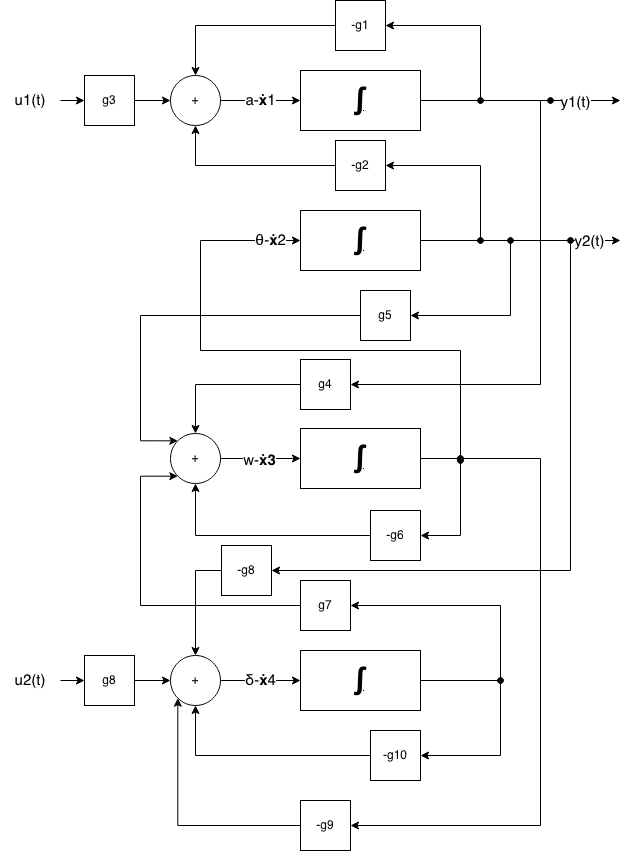
\includegraphics[width=\columnwidth]{imgs/TSII - Simulation Diagram.drawio.png}
\caption{Simulation diagram of the rocket system.}
\label{fig:simdiagram}
\end{figure}

\begin{table}[H]
\centering
\caption{Traducción de símbolos}
\begin{tabular}{|c|c|}
\hline
Símbolo & Valor \\
\hline
$g_1$ & $(1 + K_1 k_a)/\tau_m$ \\
$g_2$ & $c_\theta$ \\
$g_3$ & $K_1 k_a/\tau_m$ \\
$g_4$ & $k_\epsilon$ \\
$g_5$ & $\mu$ \\
$g_6$ & $a_d$ \\
$g_7$ & $k_\delta$ \\
$g_{10}$ & $1/\tau_s$ \\
$g_8$ & $K_2/\tau_s$ \\
$g_9$ & $\lambda K_2/\tau_s$ \\
\hline
\end{tabular}
\end{table}

pendiente de generar análisis de trayectorias y valires de K1

\subsection{Seccion A3}
Vector de estados y de entradas:
\begin{equation*}
\mathbf{x}(t)=\begin{bmatrix}x_1\\x_2\\x_3\\x_4\end{bmatrix}=\begin{bmatrix}a(t)\\\theta(t)\\\omega(t)\\\delta(t)\end{bmatrix},\qquad
\mathbf{u}(t)=\begin{bmatrix}u_1(t)\\u_2(t)\end{bmatrix}
\end{equation*}

Ecuaci\'on de estados $\dot{\mathbf{x}}(t)=A\mathbf{x}(t)+B\mathbf{u}(t)$:
\begin{equation*}
\resizebox{\columnwidth}{!}{$
\begin{bmatrix}\dot a\\\dot\theta\\\dot\omega\\\dot\delta\end{bmatrix}=
\begin{bmatrix}
-\frac{1+K_1k_a}{\tau_m} & -c_\theta & 0 & 0\\
0 & 0 & 1 & 0\\
k_\epsilon & \mu & -a_d & k_\delta\\
0 & -\frac{K_2}{\tau_s} & -\frac{\lambda K_2}{\tau_s} & -\frac{1}{\tau_s}
\end{bmatrix}
\begin{bmatrix}a\\\theta\\\omega\\\delta\end{bmatrix}+
\begin{bmatrix}
\frac{K_1k_a}{\tau_m} & 0\\
0 & 0\\
0 & 0\\
0 & \frac{K_2}{\tau_s}
\end{bmatrix}
\begin{bmatrix}u_1\\u_2\end{bmatrix}
$}
\end{equation*}

\subsection{Seccion A4}
\begin{equation*}
G_{ij}(p)=\frac{N_{ij}(p;K_1,K_2)}{D(p;K_1,K_2)},\qquad D(p)=\det(pI-A)
\end{equation*}

\begin{align*}
D(p)&=p^4+p^3(0.069902K_1+21.417)\\
&\quad+p^2(1.4225K_1+102.0K_2+27.518)\\
&\quad+p(7.13K_1K_2+0.40543K_1+278.85K_2-16.633)\\
&\quad+11.883K_1K_2-1.6776K_1+181.42K_2-2.0688\\
N_{11}(p)&=0.0034951K_1(2040.0K_2p+3400.0K_2\\
&\quad+20.0p^3+407.0p^2+116.0p-480.0)\\
N_{12}(p)&=-1667.7K_2\\
N_{21}(p)&=0.0083882K_1(p+20.0)\\
N_{22}(p)&=0.000136K_2(87377.0K_1+1.25\cdot10^{6}p+1.334\cdot10^{6})
\end{align*}

Para $K_1=1,\ K_2=0.5$:
\begin{equation*}
D(p)=p^4+21.487p^3+79.94p^2+126.76p+92.907
\end{equation*}


\subsection{Tabla de datos}
\begin{table}[H]
\centering
\caption{Ejemplo de Tabla con datos}
\label{DataTable1}
\begin{tabular}{|c|c|}
\hline
X [s] & Y[m/s]  \\
\hline
11.7 & 37.8              \\
17.1 & 54     \\  
8.4 & 26.6 \\
6.6 & 21.2 \\
7.4 & 23.4 \\
1.9 & 7   \\
\hline   
\end{tabular}
\end{table}

%EJEMPLO DE COMO UTILIZAR LOS PAQUETES PARA CREAR UNA GRAFICA
\subsection{Gr\'aficas}
\begin{figure}[H]
	\centering
	\begin{tikzpicture}
		\begin{axis}[
   			title=Puntos obtenidos,	%Title of graph
   			xlabel={x[s]},			%label the x-axis
  			ylabel={y[m/s]},		%label the y-axis
   			legend pos=south east,	%put slope legend in bottom right corner
]
			\addplot[blue, only marks] table[col sep=comma] {data/CircleData.csv};	%plot points from data table
			\addplot [red] table[col sep=comma, y={create col/linear regression={y=y}}]   %best fit line
        {data/CircleData.csv};
       
			\addlegendentry{slope=$\pgfmathprintnumber{\pgfplotstableregressiona}$}        
        %show slope value
		\end{axis}
	\end{tikzpicture}
	\caption{Ejemplo de gr\'afica}\label{diagram1}   %caption the graph
\end{figure}


\subsection{Section D.11}
The observability matrix $\mathcal{O}=[C;\ CA;\ CA^2;\ CA^3]$ has rank 4 with both sensors, with the accelerometer only, and with the pitch angle only (Table~\ref{tab:obs}), so $\omega$ and $\delta$ can be reconstructed without measuring them, using an observer. The smallest singular value $\sigma_{\min}$ shows how strong each path is. The accelerometer ``hears'' the tilt through the gravity term $-c_\theta\theta$, which is a strong path. The IMU sees the thrust only through the small misalignment $k_\varepsilon$, which is a weak path. If those couplings did not exist ($c_\theta=0$ or $k_\varepsilon=0$), observability would be lost. In an unobservable system an unstable mode could grow without being seen by the sensors, and the computer would correct based on a wrong state.

\begin{table}[H]
\centering
\caption{Observability ($K_1=1$, $K_2=0.5$)}
\label{tab:obs}
\begin{tabular}{|c|c|c|}
\hline
Sensors & rank $\mathcal{O}$ & $\sigma_{\min}(\mathcal{O})$ \\
\hline
$a$ and $\theta$ & 4 & 1.17 \\
$a$ only & 4 & 0.99 \\
$\theta$ only & 4 & 0.026 \\
$a$ only, $c_\theta=0$ & 1 & 0 \\
$\theta$ only, $k_\varepsilon=0$ & 3 & 0 \\
\hline
\end{tabular}
\end{table}

\subsection{Section D.12}
The controllability matrix $\mathcal{C}=[B\ AB\ A^2B\ A^3B]$ was evaluated in each scenario (Table~\ref{tab:ctrb}). With $u_1$ only, the rank is still 4 because the throttle reaches the attitude through $k_\varepsilon$, but the authority is minimal ($\sigma_{\min}$ about 900 times smaller): $10\,\text{\%}$ of thrust tilts the rocket only $1.03^\circ$. If the servo is physically jammed ($\dot\delta=0$), or if $K_2=0$, the rank drops to 3 and the nozzle deflection $\delta$ is out of reach; in both cases the rocket is also unstable (pole $+0.557$~s$^{-1}$). An uncontrollable state cannot be moved by any control law, so losing the nozzle is the most critical failure.

\begin{table}[H]
\centering
\caption{Controllability scenarios}
\label{tab:ctrb}
\begin{tabular}{|c|c|c|c|}
\hline
Scenario & rank & out of reach & stable \\
\hline
$u_1$ and $u_2$ & 4 & --- & yes \\
$u_1$ only & 4 & --- & yes \\
Jammed servo & 3 & $\delta$ & no \\
$u_2$ only & 4 & --- & yes \\
$K_2=0$ & 3 & $\delta$ & no \\
\hline
\end{tabular}
\end{table}

Fig.~\ref{fig:simK20} shows this in the interactive simulation of the rocket (\texttt{cohete-cabeceo.html}). With the preset $K_2=0$, the badge reports the unstable pole $+0.557$~s$^{-1}$; after $3.5$~s the rocket has pitched $26.9^\circ$ while the nozzle gauge stays at $0.00^\circ$.

\begin{figure}[H]
\centering
\includegraphics[width=\columnwidth]{imgs/sim_D_a_K2_0.png}
\caption{Simulation with $K_2=0$: unstable rocket and frozen nozzle (left gauge $\delta$, right gauge $a$).}
\label{fig:simK20}
\end{figure}

\subsection{Section E.13}
The plane $K_1\in[0,20]$, $K_2\in[0,3]$ was swept with steps $u_2=5^\circ$ and $u_1=10\%$ (script \texttt{analisis\_DE.py}). The criteria were overshoot $M_p\le10\%$, settling time $t_s\le3$~s, steady-state pitch error $\le5\%$, nozzle excursion $\delta_{\max}\le5^\circ$, positive axial gain, and the smallest possible coupling (Fig.~\ref{fig:mapas}). Raising $K_2$ improves speed, damping and pitch accuracy, but increases the nozzle excursion. Raising $K_1$ increases the axial gain and reduces the $u_2\to a$ coupling, but increases the $u_1\to\theta$ coupling. The recommended range is
\begin{equation*}
K_1\in[4,\,6],\qquad K_2\in[1.1,\,1.4],\qquad (K_1,K_2)_{\text{rec}}=(5,\ 1.25).
\end{equation*}

%DISCUSIÓN 
%Esta sección incluye la interpretación de los resultados presentados anteriormente. Se debe incluir la explicación, analisis y comparación entre lo que ya se conoce de literatura anterior y los resultados obtenidos. También  en esta sección se deben responder las preguntas propuestas en la introducción y como se prueba o rechaza la hipotesis propuesta.
\section{Discusi\'on}
\lipsum[1-2]

%CONCLUSIÓN
%Esta sección es un resumen de lo aprendido al final de haber desarrollado el proyecto. Es una sintesís de los resultados más importantes y de lo aprendido de la teoría y la práctica.
\section{Conclusi\'on}
\lipsum[1-1]

%FORMATO APA
\begin{thebibliography}{1}

\bibitem{LabWrite}
M.~Carter, E.~Weiebe, and M.~Ferzli, \emph{LabWrite}, \url{https://www.ncsu.edu/labwrite/index_labwrite.htm}, NC~State~University, 2004.

\bibitem{Fullerton}
D.~Fullerton, \emph{APlusPhysics}, \url{http://www.aplusphysics.com/courses/regents/lab_report.html}, 2016.

\bibitem{Svoronos}
T.~Svoronos, \emph{How I Will Write My Dissertation}, \url{http://teddysvoronos.com/2014/12/26/how-i-will-write-my-dissertation-3/}, 2014.

\bibitem{Clarion}
G. Clarion, \emph{Rocklin High School}, 2009.

\end{thebibliography}

\end{document}


